%!TEX root = ../../super_main.tex

\subsection{Coverage Metrics}
\label{sec:automated_unit_test}

Our development method states that all code we develop should be made in a test-first fashion (see \secref{sec:extreme_programming}). We therefore attempted to always make test cases for all the features we implemented. Our code coverage graphs can be seen in \figref{fig:android_project_code_coverage} and \figref{fig:php_project_code_coverage}, for our Android and PHP projects respectively. The two figures look different because we use different plugins on the CI server (due to the projects being written in different programming languages). We could have used a more strict coverage metric than line coverage, but due to prioritization of feature development we have chosen not to. Other interesting and useful coverage metrics includes branch coverage. In the Android project our line coverage percentage is $\sim 43\%$, which is relatively low. %But as explained previously, this is due to the complexity of the integration tests which were manual instead. 

% In \figref{fig:android_project_code_coverage} the line coverage is represented with green while missed lines are represented with red. In \figref{fig:php_project_code_coverage} the red line is method coverage, blue is line coverage and green is total.

\begin{figure}[!htbp]
    \centering
    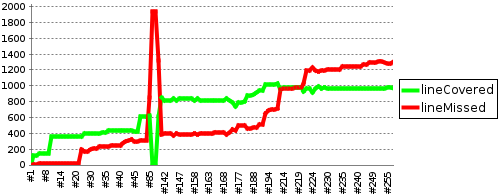
\includegraphics[width=0.7\textwidth]{graphic/quality_assurance/jenkins_android_code_coverage}
    \caption{Android project code coverage}
    \label{fig:android_project_code_coverage}
\end{figure}
\FloatBarrier

In the PHP project, we have a $\sim 74\%$ line coverage, which is rather good. Most of the untested code is library- or auto generated code, and we have not tested this because we assume these parts work as they are supposed to. This is a risk assessment we have made, and deemed insignificant, in contrast to the speed we gain from using the libraries without testing them. % If we only considered coverage on the code we made ourselves, it would probably exceed 90\%. 

\begin{figure}[!htbp]
    \centering
    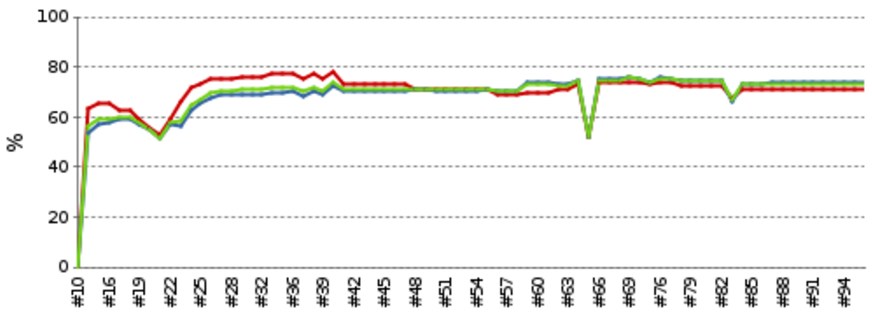
\includegraphics[width=0.7\textwidth]{graphic/quality_assurance/jenkins_php_code_coverage}
    \caption{PHP project code coverage}
    \label{fig:php_project_code_coverage}
\end{figure}
\FloatBarrier

\subsubsection{Manual Test}
In some cases it was infeasible to create automatic dynamic white box tests in decent time, and we therefore, in these cases, switched to a dynamic black box approach instead. Here we made test specifications, executed some part of the code manually and observed the result relative to the specifications. We mainly did this for the more complex parts of the code, such as the \mono{BackgroundSensorService} class, which schedules all the \mono{SensorProvider}s asynchronously and sends the results to the server. One of the manual tests for the \mono{BackgroundSensorService} is the \textbf{test-snapshot-from-device-to-server} found in \appref{app:manual_test}, which tests if our Android application correctly sends snapshots to the server, but also if the server correctly stores them. We also used this approach for other testing methods, such as regression and integration testing of UI features. For instance, we would, when a new UI-related feature was implemented, manually test if previous UI features still worked. We did not spend time on specifying written test-cases on the most basic of these tests, such as ``is it possible to subscribe to a campaign?'', since these would probably be found during ad-hoc testing while developing new features.
\newpage
These manual tests resulted in a generally lower line coverage, especially on the Android project, since the CI plugin we used was unable to compare our manual tests to the code base. This does not necessarily mean that the code is less tested, but it is harder to tell when tests are covering the code base well. 

\subsection{Static Code Analysis}
Besides using coverage metrics, we have used some metrics produced by static code analysis to improve the quality of our code base. We have used a linter, which will produce warnings on code that is known to be error prone, which helps us avoid common mistakes on the Android platform and Java in general. Furthermore, we have used check-style, which helps us find structural inconsistencies in our code base. Effectively, this type of metric will assist us in keeping our code base uniform and look consistent, which will make it easier for all developers to read the code, since all parts of the code base is structured in the same way.
